\chapter{Design and Implementation}
\label{ch:DesignImplementation}


\section{CAS Configurator Merlin}
\label{sec:DesignImplementation:ConfiguratorMerlin}

\autoref{fig:DesignImplementation:ConfiguratorMerlin} shows the architecture of CAS Configurator Merlin.
\begin{description}
    \item[M.Core] provides the base of the configurator. It checks the configuration against all rules in the database, provides possible alternatives if a change invalidates other parts of a configuration. The system relies on a CSP solver for validation and suggestion of alternatives.
    \item[M.Model] is the editor to create products and rules. These rules can then be uploaded to M.Core.
    \item[M.Customer] is the customer facing component. It allows a customer to configure a product.
\end{description}

\begin{figure}
    \centering
    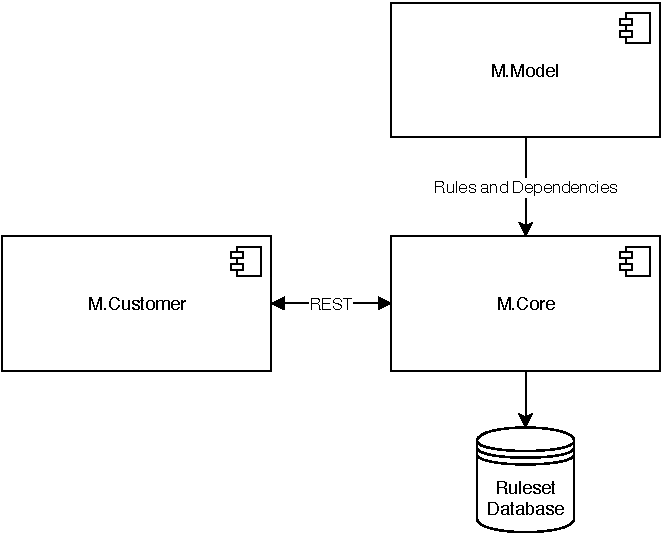
\includegraphics{./figures/50_design_and_implementation/MerlinConfigurator.pdf}
    \caption{Architecture of Configurator Merlin \cite[Fig. 4.1]{raabKollaborativeProduktkonfigurationEchtzeit2019}}
    \label{fig:DesignImplementation:ConfiguratorMerlin}
\end{figure}

\section{CAS Group-Configurator}
\label{sec:DesignImplementation:GroupConfigurator}

\citeauthor{raabKollaborativeProduktkonfigurationEchtzeit2019}'s \cite{raabKollaborativeProduktkonfigurationEchtzeit2019} extends CAS Merlin Configurator in his thesis to allow simultaneous configuration. The extended architecture is shown in \autoref{fig:DesignImplementation:CollaborativeConfiguratorMerlin}.
He only makes changes to M.Customer which is renamed to M.Collab-Customer and introduces a new component M.Collab.

\begin{description}
    \item[M.Collab] is a node.js server application that communicates with M.Core via REST-API and with M.Collab-Customer via WebSocket. It sits in between M.Collab-Customer and M.Core and handles all processing regarding collaborative configuration.
    \item[M.Collab-Customer] a modified version of M.Customer that does all communication via WebSocket and does communicate with M.Collab instead of M.Core.
\end{description}

\begin{figure}
    \centering
    \includegraphics{./figures/50_design_and_implementation/MerlinCollaborativeConfigurator.pdf}
    \caption{Architecture of Collaborative Configurator Merlin \cite[Fig. 4.3]{raabKollaborativeProduktkonfigurationEchtzeit2019}}
    \label{fig:DesignImplementation:CollaborativeConfiguratorMerlin}
\end{figure}


\section{Extended Configurator}
\label{sec:DesignImplementation:ExtendedConfigurator}

Extending \citeauthor{raabKollaborativeProduktkonfigurationEchtzeit2019} \cite{raabKollaborativeProduktkonfigurationEchtzeit2019} work a module called M.Recommender is added. Its aim is to provide a recommendation server that holds all the data needed for recommendations. M.Collab and M.Collab-Customer have to be modified to allow taking in preferences and to show  recommendations. The recommender engine is set up to be in a separate system which allows the easier replacement and the usage of different technologies. The extended architecture is shown in \autoref{fig:DesignImplementation:RecommenderForCollaborativeConfiguratorMerlin}.

\begin{description}
    \item[M.Recommender] is a new system that will get queried from M.Collab for recommendations, when the configuration changes. M.Recommender will return recommendations which then can be presented to users by M.Collab-Customer.
\end{description}

\begin{figure}
    \centering
    \includegraphics{./figures/50_design_and_implementation/MerlinCollabRecommender.pdf}
    \caption{Architecture of Collaborative Configurator Merlin with an added recommender system.}
    \label{fig:DesignImplementation:RecommenderForCollaborativeConfiguratorMerlin}
\end{figure}

\begin{figure}
    \centering
    \includegraphics[width=1\textwidth]{./figures/50_design_and_implementation/user_interface_prototype.png}
    \caption{The user interface of the prototype, seen by one user while configuring with three other people.}
    \label{fig:DesignImplementation:UserInterface}
\end{figure}


\missingfigure{Figure showing screenshot of configurator UI}